\documentclass[12pt]{article}
\usepackage[spanish]{babel}
\usepackage{graphicx}
%opening
\title{\textit{\underline{Trabajo Práctico Protocolo IPv6}}}
\author{\textbf{Valentino Aviani y Luca Mamani}}
\author{\textbf{Valentino Aviani y Luca Mamani} \\ \textbf{5to Informática}}
\begin{document}

\maketitle

\begin{abstract}
Enlace al repositorio git: https://github.com/valentinoaviani14/redes.git 

carpeta de imágenes: tpipv6/imagenes
\end{abstract}

\section{IPv6 SLAAC and EUI-64 Basics}
\subsection{Relación entre MAC y LLA según el algoritmo EUI-64}
En este caso la dirección MAC original de la PC0 es 00D0.D344.359B y la dirección Link-Local-Address (LLA) de la PC es FE80::2D0:D3FF:FE44:359B. Por otro lado, EUI-64 es un mecanismo que permite generar automáticamente una dirección IPv6 basada en la dirección MAC de un dispositivo, asegurando que cada dispositivo tenga una dirección única en su red local.
\subsection{Simulation Panel First Message}
Después de abrir el PDU para obtener detalles los campos relevantes del mensaje tipo RS (Router Solicitation) son:

1-TYPE:0x85 
 
2-CODE:0x00

3-CHECKSUM:0x0000 

4-RESERVED

5-OPTION 

Por otro lado los campos relevantes del mensaje tipo RA (Router Advertizing) son:

1-TYPE:0x86 

2-CODE:0x00

3-CHECKSUM:0x0000 

4-Hop Limit:0x40 

5-RESERVED

6-Router Lifetime:0x0708 

7-Reachable Time:0x00000000 

8-Retrans Timer:0x00000000

\subsection{GUA (Global Unicast Address)}
La PC0 a través de RS, está solicitando información a cualquier router en la red. El router anuncia a través de RA que en esta red se usa el prefijo 2001:DB8:1::/64. Dado el prefijo la PC0 genera su dirección GUA combinándolo con su indentificador EUI-64. La PC0 ahora tiene la dirección GUA 2001:DB8:1::2D0:D3FF:FE44:359B obtenida a través de SLAAC.

\section{Neighbor Discovery}
\subsection{Local Delivery}
(P1) Los mensajes NDP aparecen en la lista de eventos porque PC0 necesita conocer la dirección MAC de PC1 antes de poder enviar el ping. Esto es necesario en IPv6 ya que no se dispone del protocolo ARP de IPv4.

(P2) El primer evento ICMPv6 en PC0 es un mensaje de tipo (Echo Request) de Capa 3 o L3. Por otro lado, en L2 aparece la dirección MAC del siguiente salto, ya que para enviar un paquete la PC necesita esta dirección.

(P3) PC0 aún no conoce la MAC de PC1, para eso, usa una dirección especial de multidifusión en L2 (33:33:FF:XX:XX:XX). Después del envió del mensaje de multidifuión, PC0 aprende la dirección MAC de PC1 y ahora puede enviar paquetes directamente sin usar multicast. Con esto IPv6 evita el envío de tráfico innecesario a todos los dispositivos de la red evitando congestión en la misma.

(P4) Entre las entradas y salidas en L2 en el switch0 no hay diferencias, esto se debe a que el switch conoce la MAC destino y la entrada y salida serán iguales en Capa 2, excepto por el puerto por el que se reenvía.

(P5) Valores de las siguientes direcciones:

1 \textbf{Ethernet Destination Address:} 3333.FF00.000B

2 \textbf{Ethernet Source Address:} 0090.0C5B.E7DC

3 \textbf{IPv6 Source Address:} 2001:DB8:ACAD:1::B

4 \textbf{IPv6 Destination Address:} FF02::1:FF00:B

(P6) Al seleccionar el  evento NDP en el RO se puede comprobar que no hay información en Out Layers, esto se debe a que el paquete no ha sido reenviado y sigue en análisis interno en el router.

(P7) Sí podemos afirmar que PC0 tiene la información suficiente como para comunicarse con PC1 ya que esta comprobando conectividad con el destino.

(P8) El último evento ICMPv6 de PC0 es un mensaje de tipo Echo Request, esto implica que PC0 esta enviando un mensaje de prueba a PC1.

(P9)  No hay eventos NDP porque la dirección MAC de PC1 ya está almacenada en la de vecinos de PC0. Por otra parte, el switch también recuerda las direcciones MAC aprendidas, evitando la necesidad de reenvió de mensajes de tipo NDP.

\subsection{Non Local Delivery}
 
 (P1) Borramos la información de vecindad del router0 que quedo registrada de la seccion anterior.
 
 (P2) Como dice en el trabajo práctico, se realizó un ping a la pc2 desde la pc0.
 
 (P3) En el primer evento registrado de la simulacion, se realizo un mensaje ICMPv6 de tipo echo Request en pc0, en el cual se observa que no hay informacion de L2.
 
 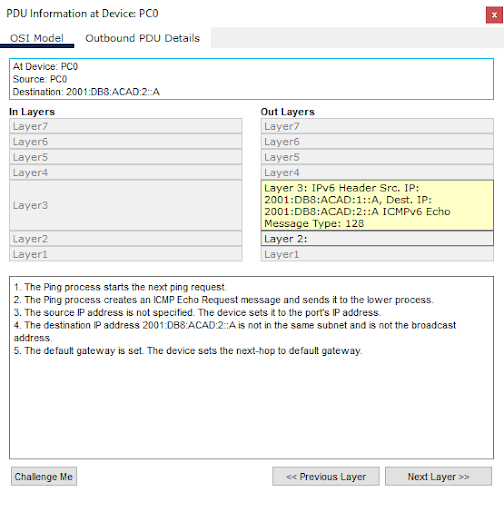
\includegraphics[width=0.7\textwidth]{../tpipv6/imagenes/imagen1}
 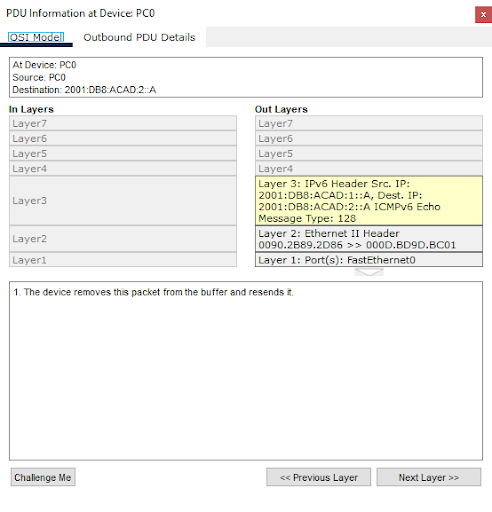
\includegraphics[width=0.7\textwidth]{../tpipv6/imagenes/imagen2}
 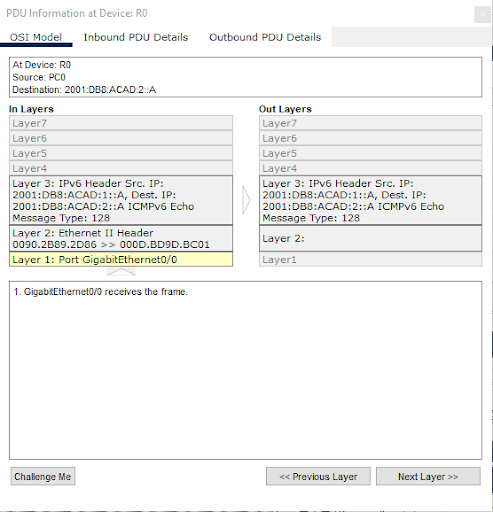
\includegraphics[width=0.7\textwidth]{../tpipv6/imagenes/imagen3}
 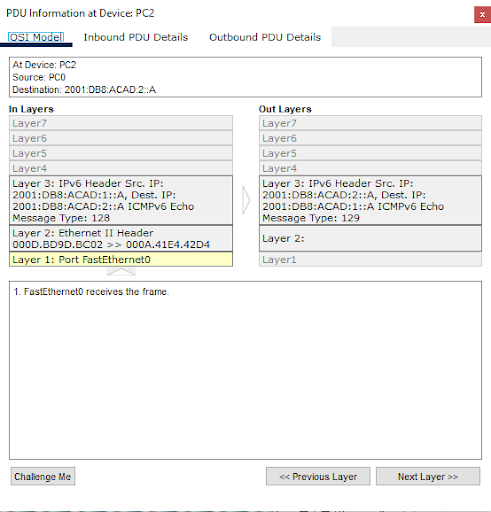
\includegraphics[width=0.7\textwidth]{../tpipv6/imagenes/imagen4}
 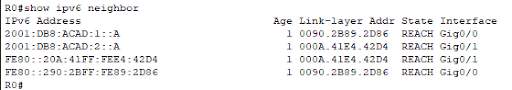
\includegraphics[width=0.7\textwidth]{../tpipv6/imagenes/imagen5}
 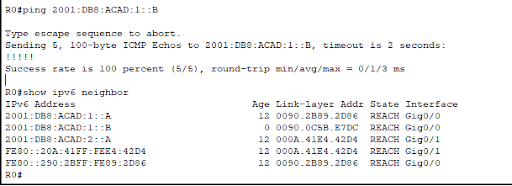
\includegraphics[width=0.7\textwidth]{../tpipv6/imagenes/imagen6}
 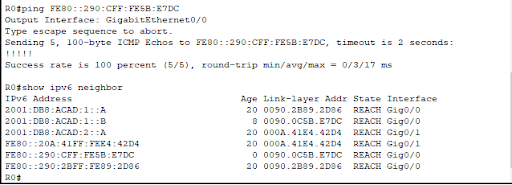
\includegraphics[width=0.7\textwidth]{../tpipv6/imagenes/imagen7}
 
\end{document}
